%
% Capítulo 2
%
\chapter{Sistema de Gestão de Stocks} \label{cap2}

O sistema de gestão de stocks desenvolvido neste projeto, denominado Smart Stocks, é apresentado neste capítulo, bem como os requisitos funcionais, não funcionais e opcionais. São ainda expostos conceitos básicos importantes para uma melhor compreensão do sistema desenvolvido.

\section{Conceitos Básicos de Gestão de Stocks} \label{sec21}
% Contador de Exemplos
\newcounter{ExampleCounter}
Em qualquer gestão de stocks é necessário realizar uma catalogação, de forma regular, dos bens ou propriedades tangíveis existentes. A essa lista dá-se o nome de \textbf{Inventário}~\cite{businessDictionary:invetoryDefinition2018}. Quando há uma forma automatizada de dar entrada e saída dos bens, o inventário serve para determinar erros e não-conformidades. 
Cada bem é identificado no stock por um código, cujo nome se dá \textbf{\acrfull{sku}} (Unidade de Manutenção de Stock, em Português)~\cite{investopedia:skuDefinition2018}. Esse código de identificação é muitas vezes retratado como um código de barras legível por máquinas que ajuda a rastrear o item para inventários. Note-se que um SKU não identifica o bem tangível, mas antes todos os bens que contêm as mesmas características. No exemplo~\ref{sec21}.1. está ilustrado um SKU.\\[0.25cm]

\stepcounter{ExampleCounter}
\noindent\fbox{
	\parbox{\textwidth}{
		\textbf{Exemplo \arabic{ExampleCounter}}\\
		Imagine-se um armário com:
		\begin{itemize}
		    \item 2 pacotes de leite magro da marca X;
		    \item 2 pacotes de leite magro da marca Y;
		    \item 1 pacote de leite meio gordo da marca X.
		\end{itemize} 
		Esse armário contém 3 \acrshort{sku}s, uma vez que um \acrshort{sku} se distingue pelo tamanho, cor, sabor, marca, etc.
	}
}\\[0.25cm]

Os itens que se mantêm em stock físico na loja são identificados como \textbf{Stock Item (Item em Stock, em Português)} \cite{sphereoi:itemIdentification2018}. O item em stock tem uma quantidade associada, e de cada vez que uma venda é feita a sua quantidade é reduzida. Ler mais em \cite{phostersoft:stockItemDefinition2018}.
A taxonomia de classificação que subdividem um setor ("yet another market construct") nos diferentes tipos de produtos para os quais existe demanda denomina-se por \textbf{Category (Categoria, em Português)}. Quanto mais especializada for uma categoria, mais especializado é o produto.

{\footnotesize Nota: Neste projeto apenas se consideram as categorias de maior dimensão, são elas, por exemplo, Laticínios, Bebidas, Frescos, Congelados, entre outras.}

Como distinção de produtos entre empresas, recorre-se a um símbolo de identificação, marca, logótipo, nome, palavra e/ou frase, a que se dá o nome de \textbf{Brand (Marca, em Português)} \cite{investopedia:brandDefinition2018}.
Quando os estrategistas de marca falam sobre \textbf{Segmentation (Segmento, em Português)}, referem-se à segmentação do consumidor/audiência. A maneira antiga de abordar isto era através da demografia (idade, sexo, etnia, faixa de renda, urbano-rural, etc.). Agora a segmentação é VALS (valores, atitudes e estilo de vida). Ler mais em \cite{sphereoi:itemIdentification2018}.

{\footnotesize Nota: Neste projeto o segmento é a quantidade presente numa embalagem, i.e., para um pacote de leite de 1L, o segmento é 1L.}

A \textbf{Variety (Variedade, em Português)} é confusa porque pode ser difícil de entender onde a especialização do segmento termina e a especialização em prol da variedade começa. A variedade é sobre a personalização de um produto para se adequar ao caráter do consumidor individual. Ver exemplo \ref{sec21}.2. Ler mais em \cite{sphereoi:itemIdentification2018}.\\[0.25cm]

\stepcounter{ExampleCounter}
\noindent\fbox{
	\parbox{\textwidth}{
		\textbf{Exemplo \arabic{ExampleCounter}}\\	
		Note-se um pacote de leite com as caraterísticas, quantidade líquida igual a 1L, da marca X e do tipo UHT magro. Então, identificar-se-ia da seguinte forma: 
		\begin{itemize}
			\item Categoria: Laticínios
			\item Produto: Leite
			\item Marca: X
			\item Segmento: 1L
			\item Variedade: UHT Magro
		\end{itemize}
	}
}

%\vspace{0.2cm}
%\textbf{Stock Item (Item em Stock, em Português)} - Refere-se aos itens que se mantêm em stock físico na loja. O item em stock tem uma quantidade associada, e de cada vez que uma venda é feita a sua quantidade é reduzida. Ler mais em \cite{phostersoft:stockItemDefinition2018}.

%\vspace{0.2cm}
%\textbf{Category (Categoria, em Português)} - Taxonomia de classificação que subdividem um setor ("yet another market construct") nos diferentes tipos de produtos para os quais existe demanda. Quanto mais especializada for uma categoria, mais especializado é o produto. Ler mais em \cite{sphereoi:itemIdentification2018}.

%{\footnotesize Nota: Neste projeto apenas se consideram as categorias de maior dimensão, são elas, por exemplo, Laticínios, Bebidas, Frescos, Congelados, entre outras.}

%\vspace{0.2cm}
%\textbf{Brand (Marca, em Português)} - Um símbolo de identificação, marca, logótipo, nome, palavra e/ou frase que as empresas usam para distinguir os seus produtos dos outros. Ler mais em \cite{investopedia:brandDefinition2018}

%\vspace{0.2cm}
%\textbf{Segmentation (Segmento, em Português)} - Quando os estrategistas de marca falam sobre segmento, referem-se à segmentação do consumidor/audiência. A maneira antiga de abordar isto era através da demografia (idade, sexo, etnia, faixa de renda, urbano-rural, etc.). Agora a segmentação é VALS (valores, atitudes e estilo de vida). Ler mais em \cite{sphereoi:itemIdentification2018}.

%{\footnotesize Nota: Neste projeto o segmento é a quantidade presente numa embalagem, i.e., para um pacote de leite de 1L, o segmento é 1L.}


%\vspace{0.2cm}
%\textbf{Variety (Variedade, em Português)} - A variedade é confusa porque pode ser difícil de entender onde a especialização do segmento termina e a especialização em prol da variedade começa. A variedade é sobre a personalização de um produto para se adequar ao caráter do consumidor individual. Ver exemplo \ref{seca21}.2. Ler mais em \cite{sphereoi:itemIdentification2018}.

%\vspace{0.5cm}

%
% Secção 2.2
%
\section{Sistema Smart Stocks} \label{sec22}
Smart Stocks é um sistema que visa dar suporte à gestão de stocks domésticos. Para tal é necessário recolher determinadas informações, tais como, as características da casa a gerir, as particularidades dos membros co-habitantes da casa e ainda os padrões de consumo e reposição. De forma a facilitar tal tarefa são disponibilizadas listas geridas pelo sistema. Por exemplo, lista de compras e lista dos itens em stock na casa, cuja consistência é garantida às custas dos movimentos de entrada e saída dos itens nos diversos locais de armazenamento.

%
% Subsecção 2.2.1
%
\subsection{Requisitos} \label{subsec221}
Como forma de assegurar as funcionalidades pretendidas para o sistema, são exigidos os seguintes requisitos funcionais e opcionais.

\paragraph{Requisitos Funcionais}
\begin{itemize}
	\item Informar o utilizador dos itens existentes, a sua validade e a sua quantidade;
	\item Alertar sobre os produtos que estão perto do fim;
	\item Gerar listas de compras com os produtos em falta;
	\item Possibilidade de criar listas com produtos e suas quantidades;
	\item Partilhar listas entre utilizadores da mesma casa;
	\item Especificar alergias dos membros da casa.
\end{itemize}

\paragraph{Requisitos Não Funcionais}
\begin{itemize}
	\item Desenhar interfaces com o utilizador de fácil utilização;
	\item Desenhar interfaces com o utilizador com design apelativo;
	\item Internacionalizar as interfaces com o utilizador.
\end{itemize}

\paragraph{Requisitos Opcionais}
\begin{itemize}
	\item Criar listas de produtos quase a expirar;
	\item Criar listas de produtos indesejados (Lista Negra);
	\item Criar listas de contenção em situações de emergência (Lista SOS);
	\item Inserir refeições extraordinárias de eventos a realizar num futuro próximo, para acrescentar alimentos não básicos à lista de compras.
	\item Notificar o utilizador da proximidade do fim da data de validade de um determinado produto.
	\item Notificar o utilizador para a rotura iminente da quantidade de um determinado produto.
\end{itemize}

%
% Secção 2.3
%
\section{Arquitetura da Solução}\label{sec23}

Nesta secção pretende-se abordar de forma geral a solução implementada para resolver o problema apresentado no capítulo \ref{cap1}.

%
% Subsecção 2.3.1 Abordagem
%
\subsection{Abordagem}\label{subsec231}

\begin{figure}[H]
	\centering
	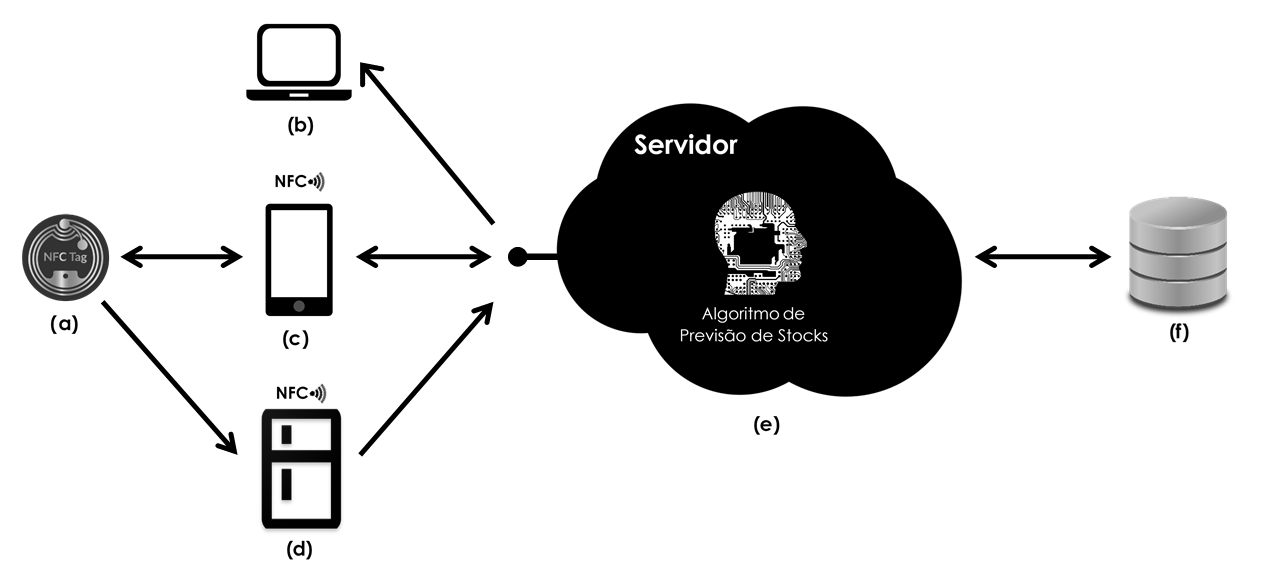
\includegraphics[width=16cm, height=8cm, scale=1]{img/architecture.png}
	\caption{Arquitetura Geral do Projeto}
	\label{project-general-architecture}
\end{figure}

Após uma ida às compras, os itens adquiridos com rótulos não tradicionais, Figura \ref{project-general-architecture}(a), são armazenados nos seus respetivos locais, Figura \ref{project-general-architecture}(d). Como forma de automatizar a recolha de informação relativa quer aos artigos obtidos quer às suas caraterísticas, utilizam-se rótulos digitais e sensores.

Ao guardar os artigos nos locais de armazenamento, os seus rótulos devem ser lidos por dispositivos de hardware, conjunto sensor mais leitor de rótulos digitais, presentes no local, de forma a que a informação e identificação do item, bem como, o tipo de movimento (entrada ou saída) possam ser enviados para a componente servidora, Figura \ref{project-general-architecture}(e). Assim, estes dados são posteriormente tratados e armazenados de forma persistente na \acrfull{bd}, Figura \ref{project-general-architecture}(f). A componente servidora é responsável por retornar dados para as aplicações cliente, Figura \ref{project-general-architecture}(b, c). É ainda nesta que está presente o algoritmo de previsão de stocks utilizado para efetuar a previsão quanto à duração de cada um dos itens em stock, assim como, o controlo da gestão de stocks.

No contexto da gestão de stocks assume-se a existência de duas formas de apresentação para os itens em stock: avulsos e embalados. Os primeiros são conservados em sistemas de arrumação identificados com \textit{tags} programáveis por \textit{smartphones}, \ref{project-general-architecture}(c). Os detalhes dos itens são especificados pelo utilizador e carregados para a \textit{tag}. Já os segundos contêm os seus rótulos digitais com o detalhe guardado pelos embaladores.

%
% Tags
%
%
% Tags
%
\subsection{Rótulos dos Itens em Stock}
\subsubsection{Requisitos Legais dos Rótulos}
Segundo o Regulamento (UE) nº1169/2011 \cite{asae:labeling} os rótulos devem conter a seguinte lista de informação:
\begin{itemize}
    \item Denominação da venda;
    \item Listas de ingredientes;
    \item Quantidades de ingredientes ou das categorias de ingredientes;
    \item Quantidade líquida;
    \item Data de durabilidade mínima (DDM)/ Data limite de consumo (DLM);
    \item Condições especiais de conservação e utilização;
    \item Nome ou firma e endereço fabricante, do acondicionador ou do vendedor;
    \item País de origem ou de proveniência;
    \item Instruções de utilização;
    \item Referência ao teor alcoométrico volúmico adquirido.
\end{itemize}

\subsubsection{Rótulos Tradicionais \textit{vs} Rótulos Digitais}
Os códigos de barras são amplamente utilizados na identificação de produtos, quer seja dentro da própria organização, quer seja quando a empresa produtora pretende vender os seus produtos no mercado. Neste último caso, a codificação dos produtos, sendo uma obrigação do mercado, segue as normas da organização GS1\footnote[1]{https://www.gs1.org/}, organização responsável pelo sistema de Normas Globais de Identificação e Codificação de bens e serviços mais utilizado no mundo. A GS1 Portugal é a entidade competente geradora e reguladora da atribuição dos códigos de barras em Portugal. É garantido que não existem dois produtos com o mesmo código de barras em circulação quer a nível nacional, quer a nível global. 

São três os componentes relevantes identificados por um código de barras: o país de origem, a empresa fabricante e o produto produzido, ilustrado na Figura~\ref{bar-code-example} (um exemplo fictício).

\begin{figure}[H]
	\centering
	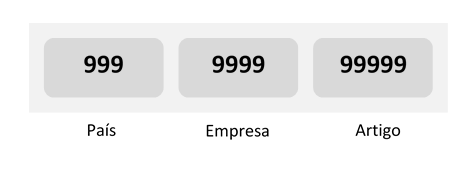
\includegraphics[scale=0.8]{img/codigo_barras_no_background.png}
	\caption{Exemplo proposto de código de barras}
	\label{bar-code-example}
\end{figure}

A gestão de stocks do sistema Smart Stocks necessita de saber o nome do produto, a marca, a variedade, o segmento, a data de validade, os alergénios, a quantidade e, opcionalmente, as condições de conservação. Logo, a informação presente nos códigos de barras é insuficiente para o correto funcionamento do sistema. Como tal, existiu a necessidade de encontrar uma nova abordagem que solucionasse o problema. Uma solução possível passa pela utilização de um leitor de imagens ou de objetos 3D, capaz de ler a informação presente no rótulo tradicional. No entanto, uma outra hipótese é a utilização de rótulos digitais, por exemplo, recorrendo a \textit{tags} \acrfull{nfc} \cite{nfcforum:nfc} ou \acrfull{rfid} \cite{rfidinc:rfid}. 
Como os produtos avulsos têm de ser rotulados, decidiu-se usar \textit{tags} programáveis por \textit{smartphones}. Este processo torna-se prático e acessível a muitos. Ora, uma vez que esta tecnologia é utilizada para os produtos avulsos e sendo uma das soluções possíveis para os produtos embalados, então, uniformiza-se a automatização utilizando a mesma tecnologia nas duas circunstâncias.

\subsubsection{Comparação entre \textit{Tags} NFC e RFID}
\begin{table}[H]
	\centering
	\caption{Comparação da tecnologia \acrshort{nfc} com a tecnologia \acrshort{rfid}}\vspace{2mm}
	\label{tab-comparacao-nfc-vs-rfid}
	\resizebox{\textwidth}{!}{%
		\begin{tabular}{m{6cm}|C{3cm}|C{3cm}}
			
			\textbf{} & \textbf{\acrshort{nfc}} & \textbf{\acrshort{rfid}} \\
			\hline Gama de frequência & 13,56MHz & 125kHz - 960MHz \\
			\hline Comunicação & Unidirecional ou bidirecional (P2P) & Unidirecional \\
			\hline Distância & até 5cm & até 100m \\
			\hline Componentes & Leitor \acrshort{nfc} e \textit{tag} \acrshort{nfc} & Leitor \acrshort{rfid}, \textit{tag} \acrshort{rfid} e uma antena \\
			\hline Suporte em \textit{smartphones} & Na maioria dos \textit{smartphones} & Não \\
			\hline Ativo/Passivo & Passivo, ativado na presença de um leitor \acrshort{nfc} & Passivo, ativado na presença de um leitor \acrshort{rfid} e Ativo, a \textit{tag} tem uma fonte de energia própria. \\
			\hline Uso aplicacional & Propriedade desenvolvidas para pagamentos móveis seguros & Usado globalmente para gestão de stocks, manipulação de bagagem no aeroporto, identificação de gado entre outros \\
			\hline Capacidade das \textit{tags} & 64 Bytes até 1024 Bytes & 96 Bits até 512 Bits ou até 4k ou 8k Bytes \\
			
		\end{tabular}
	}
\end{table}

Conforme se pode observar na tabela \ref{tab-comparacao-nfc-vs-rfid}, a comunicação com as \textit{tags} \acrshort{nfc} pode ser bidirecional o que torna mais fácil e intuitiva a transmissão entre telemóveis e \textit{tags} \acrshort{nfc}. Desta forma, optou-se pela utilização de \textit{tags} \acrshort{nfc} para os produtos avulsos em que é preciso usar o telemóvel para as programar, e, atualmente, os telemóveis só têm suporte para a tecnologia \acrshort{nfc}. Assim os locais de armazenamento têm obrigatoriamente de dispor de leitor de \textit{tags} \acrshort{nfc}. Contudo, se os embaladores decidirem utilizar \acrshort{rfid}, o hardware pode também ter leitor \acrshort{rfid}. O levantamento de requisitos feito, juntamente com a dimensão dos campos da base de dados, e sabendo que o formato utilizado na escrita das \textit{tags} é \acrlong{csv} \cite{RFC4180:csv}, estimou-se que a capacidade de armazenamento mínima das \textit{tags} é aproximadamente 324 Bytes.


\subsection{Dispositivos de \textit{Hardware}}

Posto que a componente de \textit{hardware}, sensores e leitores de \textit{tags}, não foi âmbito do projeto, mas é parte integrante e essencial para o correto funcionamento do sistema desenvolvido, foi fundamental efetuar análise e pesquisa alusiva ao assunto. Por isso, estudou-se como se deveria proceder para incorporar os dispositivos \textit{hardware} no sistema Smart Stocks. 

Assim, para adicionar um dispositivo de \textit{hardware} usar-se-ia um \textit{QRCode} \cite{qrcode:about}. Este \textit{QRCode} deveria conter informação acerca do dispositivo, como o seu identificador e possivelmente o local de armazenamento a que se destina. Este ao ser comprado e sem ter sido ainda instalado no local de armazenamento, seria adicionado à casa, pelo utilizador, recorrendo a uma funcionalidade extra da aplicação móvel. O utilizador passaria o \textit{scanner} \textit{QRCode} sobre o \textit{QRCode} presente no dispositivo de \textit{hardware} e assim a aplicação móvel comunicaria com a \gls{api-web} para associar aquele dispositivo à casa do utilizador. Caso este utilizador tenha várias casas, este teria de, previamente, especificar a qual casa pretendia associar o dispositivo. Uma vez associado, o dispositivo necessita de comunicar com a \gls{api-web} de forma a registar os movimentos presentes ocorridos naquele local de armazenamento. Para tal, quando o dispositivo for instalado e ligado, este faria um \textit{ping} à \gls{api-web} a sinalizar que está ativo e enviando a sua informação, nomeadamente o seu identificador. A \gls{api-web} respondia com o link ao qual o dispositivo \textit{hardware} teria de enviar a informação dos movimentos que deteta.

%
% Subsecção 2.3.2 Estrutura
%
\subsection{Arquitetura por Camadas}\label{subsec232}

O sistema de gestão de stocks é composto por 2 blocos principais: o bloco do lado do cliente e o bloco do lado do servidor, que se relacionam. A representação destes blocos é apresentada na Figura \ref{project-layers-structure}.

A arquitetura do projeto segue uma arquitetura por camadas, dado que este padrão permite individualizar cada camada \cite{Haque:2007:ADA:1698307.1698331}. Assim, estas tornam-se independentes umas das outras, fornecendo não só abstração sobre as camadas inferiores, mas também, oferecendo a possibilidade de testar e/ou substituir cada uma das camadas de forma independente, desde que seja mantido o contrato.

\begin{figure}[H]
	\centering
	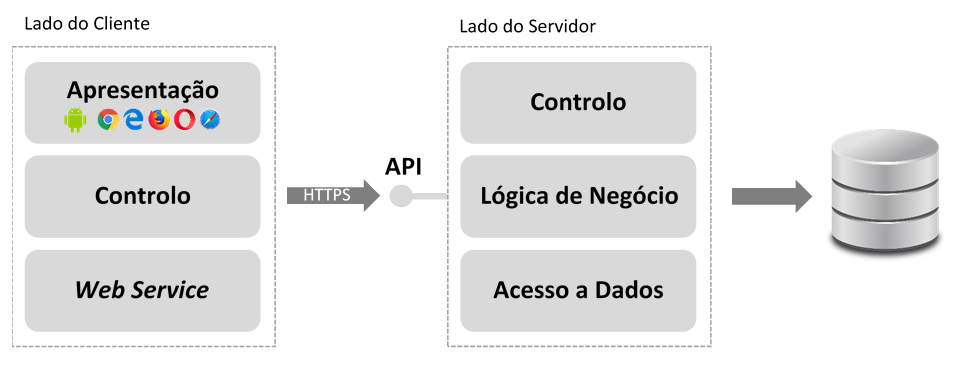
\includegraphics[width=\textwidth, scale=1]{img/project.png}
	\caption{Arquitetura por Camadas do Projeto}
	\label{project-layers-structure}
\end{figure}

No lado do cliente existem três camadas: a camada Apresentação que é responsável por representar os dados solicitados pelo utilizador; o Controlo que está encarregue de despoletar ações na camada do \textit{Web Service} de forma a satisfazer as solicitações do utilizador; e assim o \textit{Web Service} interage com a \gls{api-web}. 

As camadas que compõem o lado do servidor são: o Controlo que processa pedidos e retorna uma resposta; a camada da Lógica de Negócio que é responsável por satisfazer as regras de negócio; e por fim o Acesso a Dados que efetua leituras e escritas sobre a \acrshort{bd}.

\subsubsection{Tecnologias Inerentes à Solução}\label{subsec233}

O lado do servidor incluí três camadas e expõe uma \gls{api-web}. A \acrfull{dal} é produzida com a linguagem de programação \textit{Java}, usando a \acrfull{jpa}, e é responsável pelas leituras e escritas sobre a \acrfull{bd}. A \acrshort{bd} é externa ao servidor, utilizando para isso o \acrfull{sgbd} \textit{PostgreSQL}. A \acrfull{bll} é responsável pela aplicação das regras de negócio. A implementação desta camada é também realizada com linguagem \textit{Java}. Os \textit{controllers} foram desenvolvidos em \textit{Java} com a \textit{framework} da \textit{Spring}, chamada de \textit{Spring Boot}\footnote{https://spring.io/projects/spring-boot}. A \gls{api-web} disponibiliza recursos em diferentes \textit{hypermedias}. Para a implementação do algoritmo de previsão de stocks usou-se a linguagem \textit{R}.

Do lado do cliente existem dois modos de interação: usando uma aplicação móvel ou usando uma aplicação web. A aplicação móvel está disponível para a plataforma \textit{Android}, e foi desenvolvida na linguagem \textit{Kotlin}. A aplicação web é compatível com a maioria dos \textit{browsers}, e é implementada utilizando a linguagem \textit{JavaScript} com o auxilio da biblioteca \textit{React}\footnote{https://reactjs.org}.
%
% Subsecção 2.4
%
\section{Entidades} \label{sec24}

Em seguida identificam-se as diversas entidades relevantes que compõem o sistema de informação, que permite gerir os itens em stock numa dada casa.
\subsubsection{Casa}
\begin{itemize}
	\item Cada casa é caracterizada por um identificador único, um nome, atribuído por um utilizador no momento de registo da casa. 
	\item Deve ser possível saber o número de bebés, crianças, adultos e seniores que vivem nessa casa.
	\item Uma casa está associada a um ou mais utilizadores, podendo um utilizador ter várias casas. 
	\item Existe um ou mais administradores de uma casa.
	\item A casa pode ter vários itens em stock.
	\item Para cada casa existem vários locais de armazenamento dos itens, por exemplo armários, frigoríficos, etc.
	\item Em cada casa deve ser possível conhecer as alergias assim como quantos membros possuem essa alergia (os membros não precisam necessariamente de estar registados).
\end{itemize}

\subsubsection{Utilizador}
\begin{itemize}
	\item Uma pessoa é representada por um utilizador que é caracterizado por um email ou por um nome de utilizador, pelo nome da pessoa, a sua idade e uma \textit{password}.
\end{itemize}

\subsubsection{Listas}
\begin{itemize}
	\item Cada lista é composta por um identificador único e um nome.
	\item Uma lista pode ter vários produtos.
	\item Existem dois tipos de listas: de sistema e de utilizador. 
	\item As listas de sistema são comuns a todos os utilizadores registados, contudo são particulares a cada casa.	
	\item Um utilizador pode criar as suas listas, partilhando-as com outros utilizadores da casa ou tornando-as secretas.
\end{itemize}

\subsubsection{Categoria}
\begin{itemize}
	\item Uma categoria é identificada univocamente por um número ou por um nome.
\end{itemize}


\subsubsection{Produtos}
\begin{itemize}
	\item Um produto é constituído por um identificador único, um nome, se é ou não comestível, e a validade perecível.
	\item Para os produtos presentes numa lista pode ser possível saber a sua marca e a quantidade.
	\item Um produto pertence a uma categoria, podendo uma categoria ter vários produtos.
	\item Um produto pode ser concretizado por diversos itens em stock na casa.
\end{itemize}
 
\subsubsection{Item em Stock}
\begin{itemize}
	\item Um item em stock é a concretização de um produto que existe numa casa. É identificado univocamente por um número ou por uma marca, uma variedade e um segmento, é também caracterizado por uma descrição, o local de conservação, a quantidade e as datas de validade. 
	\item Para cada item deve ser possível saber os seus movimentos de entrada e saída de um local de armazenamento.
	\item Deve também ser possível saber os alergénios de cada item presente na casa.
\end{itemize}

\subsubsection{Movimento}
\begin{itemize}
	\item Para cada movimento deve ser possível saber o tipo do movimento (entrada ou saída), a data em que ocorreu e a quantidade de produtos. 
\end{itemize}

\subsubsection{Local de armazenamento}
\begin{itemize}
	\item Cada local de armazenamento é caraterizado por um identificador único, a temperatura e um nome.
	\item Deve ser possível saber a quantidade de cada item presente no local.
	\item Um local de armazenamento pode ter vários itens em stock presentes na casa e estar associado a diversos movimentos.
\end{itemize}